\chapter{Results and Discussion}
\label{ch:results}

\section{Data Validation against CDC}
% Counts: deaths 8/8, births 7/8 (2020 guide typo) -> FAIL by rule; Table 2 exact 2018--2023.
\todo{Write. Table: reference/benchmark_counts.csv.}

\section{Who Dies before Age One}
\begin{figure}[htbp]
  \centering
  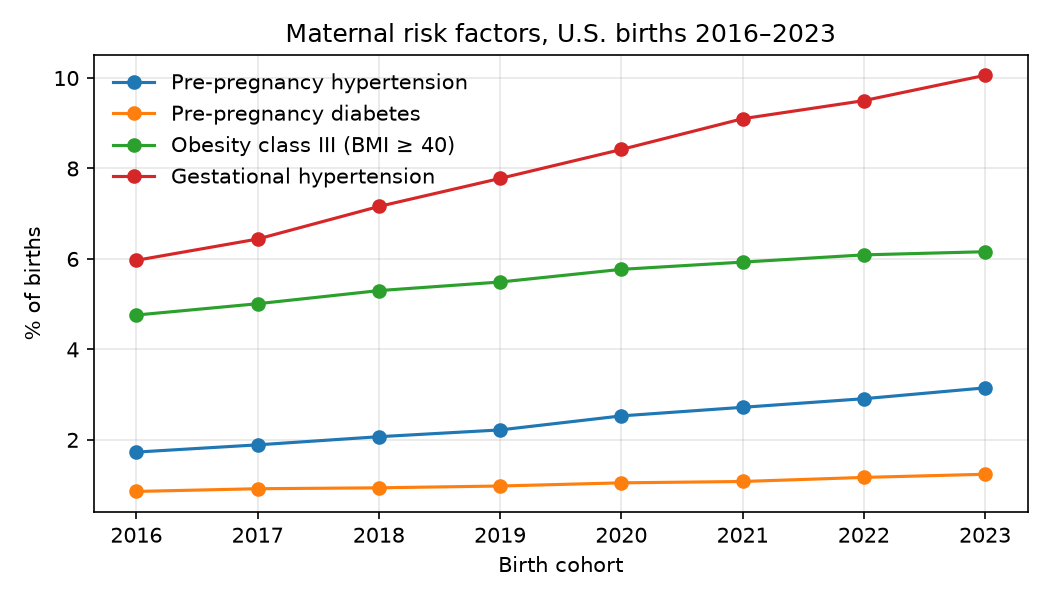
\includegraphics[width=0.85\textwidth]{risk_factor_trends.png}
  \caption{\todo{Caption that states the result.}}
  \label{fig:trends}
\end{figure}
\todo{Write. Table: reports/table1_by_outcome.csv.}

\section{Model Comparison and Calibration}
% Lead with the strict results (0.030; strict-2 0.0275) next to the pre-registered 0.038.
\begin{figure}[htbp]
  \centering
  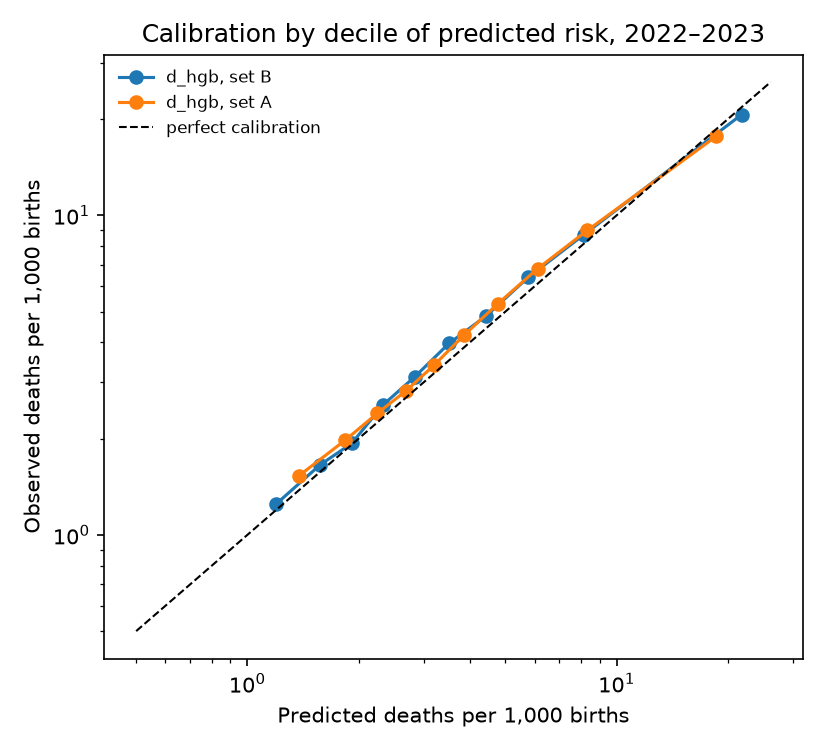
\includegraphics[width=0.75\textwidth]{part1_calibration.png}
  \caption{\todo{Caption.}}
  \label{fig:calibration}
\end{figure}
\todo{Write. Tables: reports/part1_model_comparison.csv, part1_strict.csv, part1_test_years.csv.}

\section{What Drives the Prediction}
\begin{figure}[htbp]
  \centering
  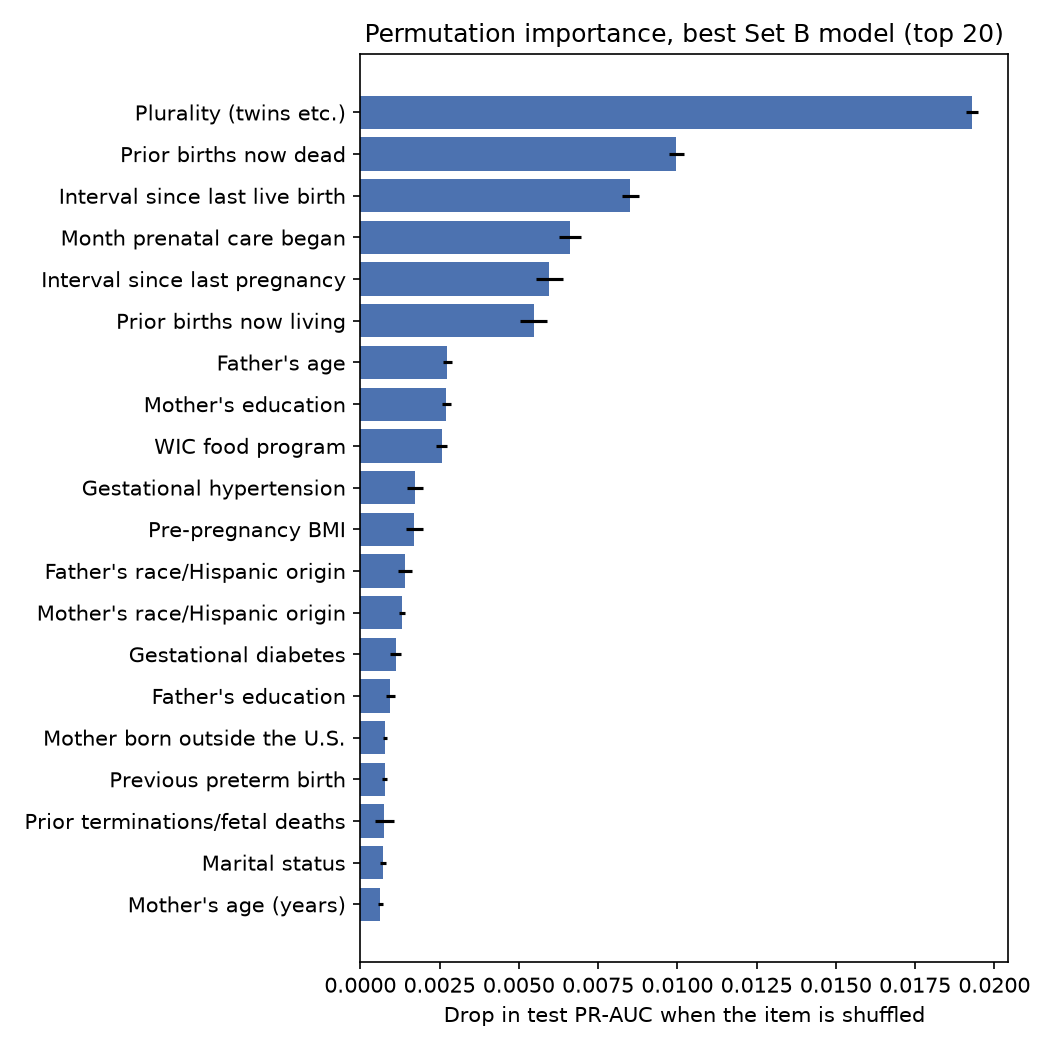
\includegraphics[width=0.85\textwidth]{part1_importance.png}
  \caption{\todo{Caption.}}
  \label{fig:importance}
\end{figure}
\todo{Write. Tables: reports/part1_importance.csv, part1_dropgroup.csv, part1_leakage.csv.}

\section{Early versus Late Deaths, Subgroups and Fairness}
\todo{Write. Tables: reports/part1_agesplit_*.csv, part1_subgroups.csv.}

\section{Decision Curves}
\begin{figure}[htbp]
  \centering
  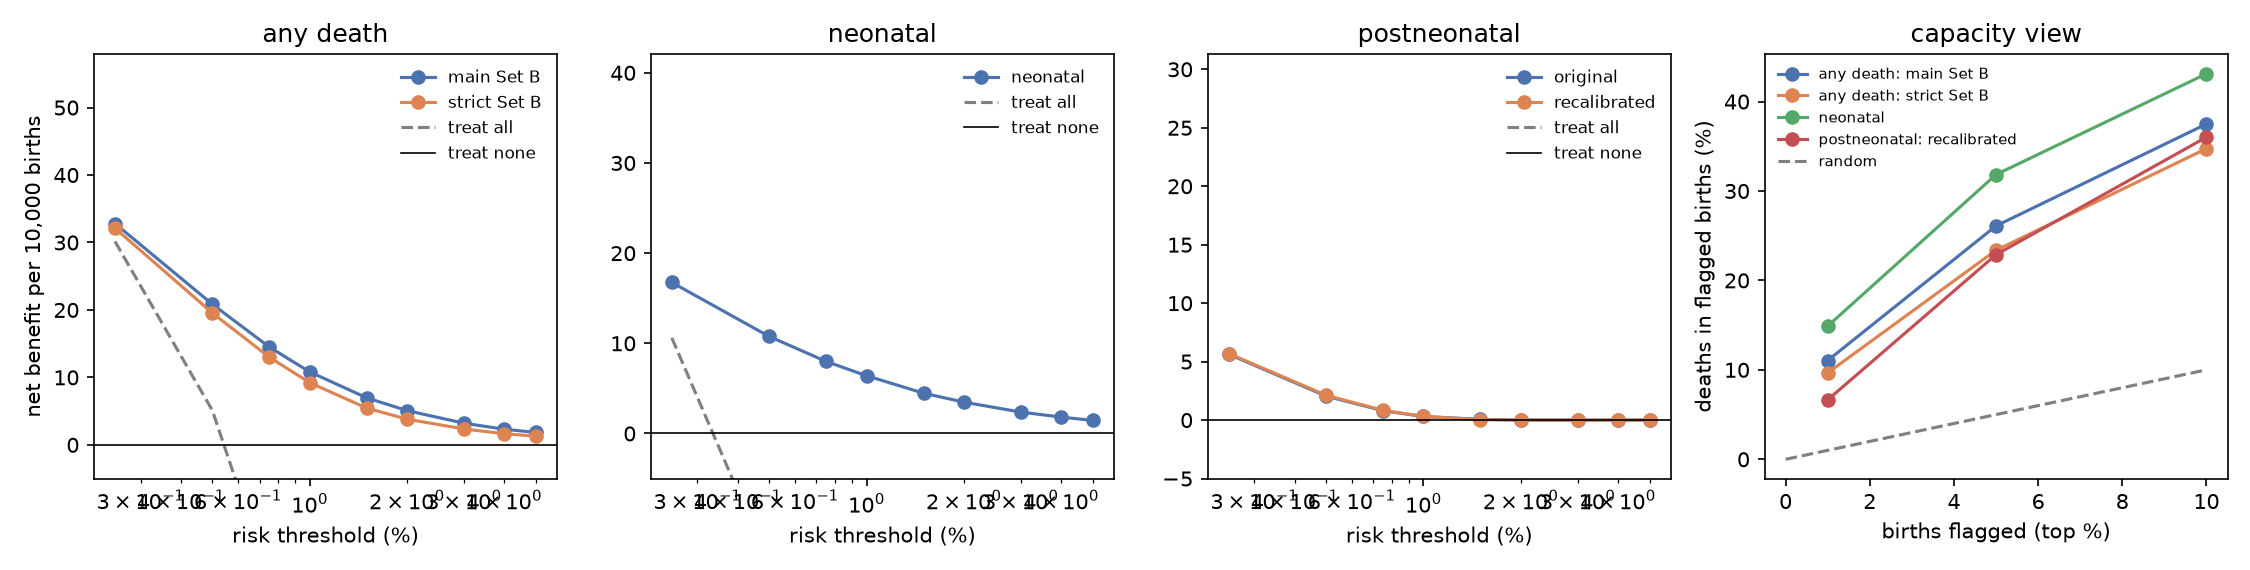
\includegraphics[width=0.85\textwidth]{extra_decision_curves.png}
  \caption{\todo{Caption.}}
  \label{fig:dca}
\end{figure}
\todo{Write. Table: reports/extra_decision_curves.csv.}

\section{Adjusted Risk Ratios for the Five Maternal Factors}
\begin{figure}[htbp]
  \centering
  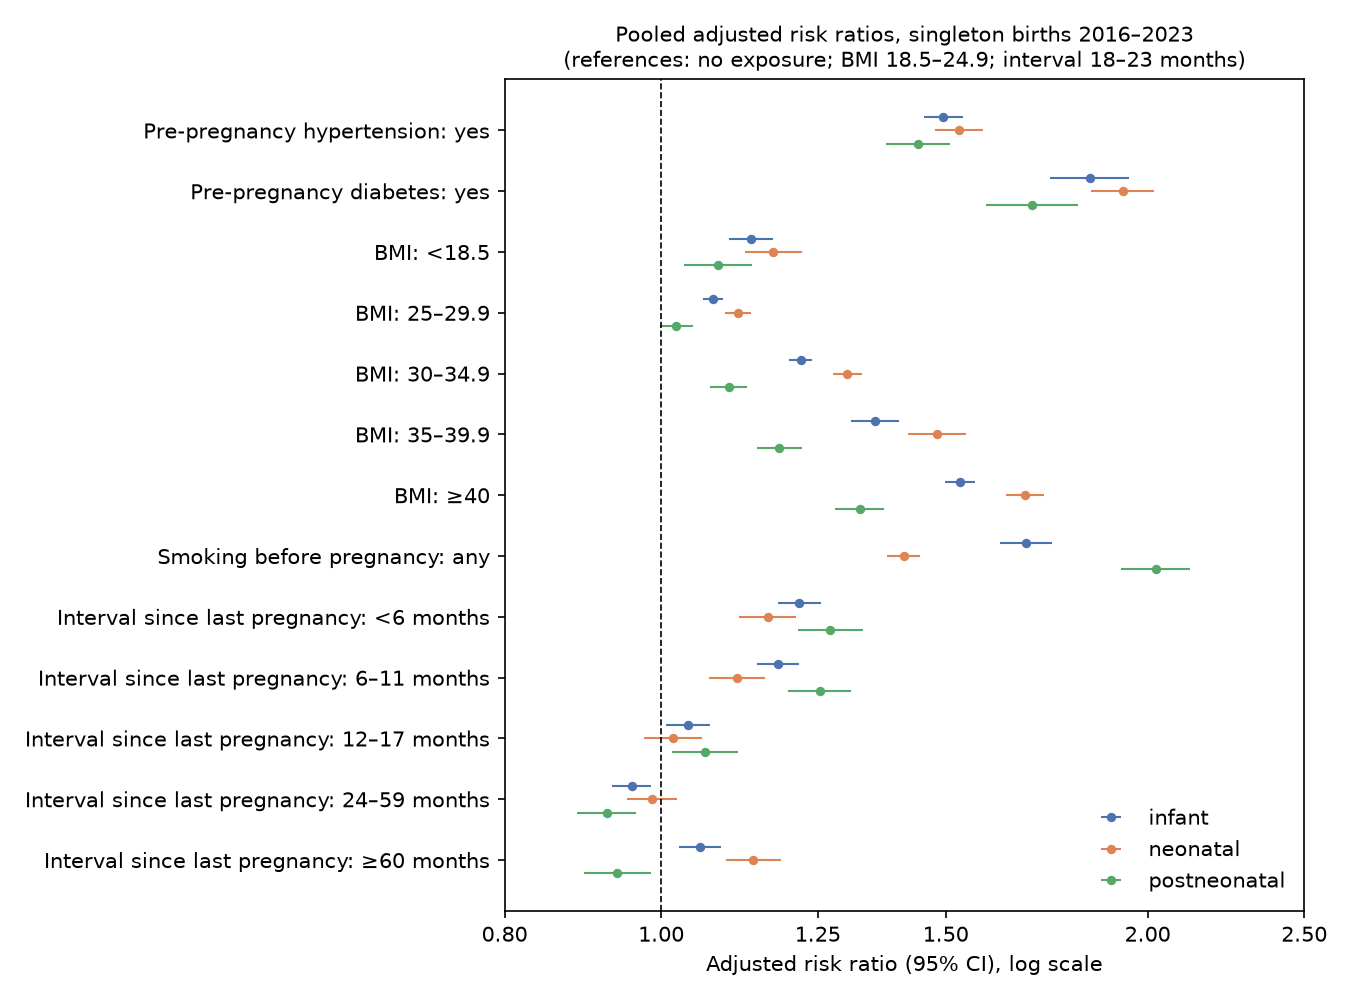
\includegraphics[width=0.85\textwidth]{part2_forest_pooled.png}
  \caption{\todo{Caption.}}
  \label{fig:forest}
\end{figure}
\todo{Write. Tables: reports/part2_results.csv, part2_exposure_counts.csv.}

\section{Robustness: Direction, Heterogeneity, Imputation and Sensitivity}
\todo{Write. Tables: reports/part2_mi_results.csv, part2_sensitivity.csv, part2_social_sensitivity.csv; figure part2_forest_by_cohort.png.}

\section{Negative Control and Collider Demonstration}
% Audit #2 (04 section 19): without codes 148--150 the smoking accident RR is still 1.59 (1.33--1.89).
\todo{Write. Tables: reports/part2_negative_control.csv, part2_collider.csv.}

\section{Cause of Death, Recording Bias and Stillbirths}
\begin{figure}[htbp]
  \centering
  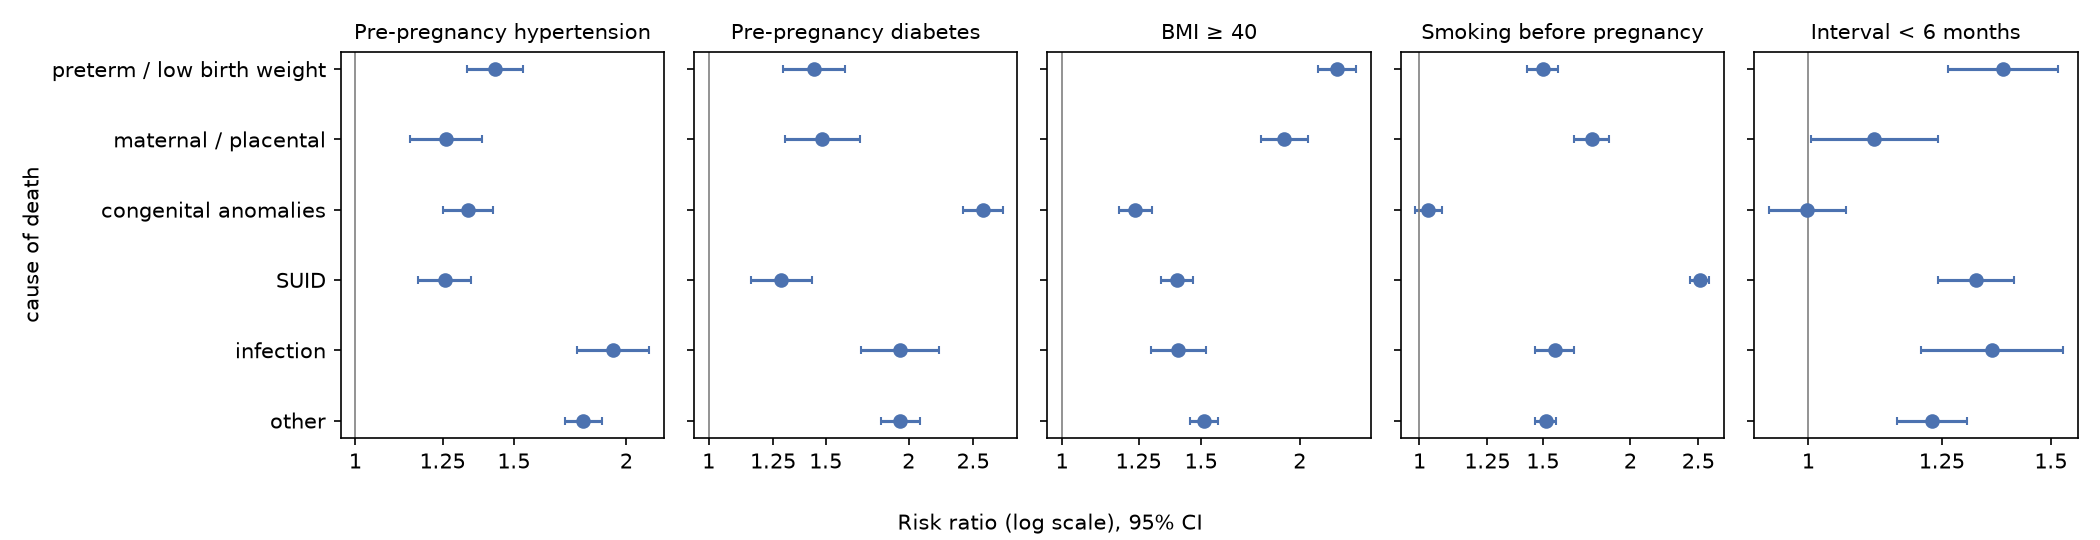
\includegraphics[width=0.85\textwidth]{extra_cause_specific.png}
  \caption{\todo{Caption.}}
  \label{fig:cause}
\end{figure}
\todo{Write. Tables: reports/extra_cause_*.csv, extra_bias_analysis.csv, extra_stillbirth.csv.}

\section{Mediation through Gestational Age}
% Audit #1 (06 section 9): report proportions mediated as upper bounds; OE hypertension direct RR 0.92 < 1.
\todo{Write. Table: reports/extra_mediation.csv.}

\section{Comparison with Published Studies}
\todo{Write.}
